% !TEX TS-program = xelatex
% !TEX encoding = UTF-8

% This is a simple template for a XeLaTeX document using the "article" class,
% with the fontspec package to easily select fonts.

\documentclass[11pt]{article} % use larger type; default would be 10pt

\usepackage{fontspec} % Font selection for XeLaTeX; see fontspec.pdf for documentation
\defaultfontfeatures{Mapping=tex-text} % to support TeX conventions like ``---''
\usepackage{xunicode} % Unicode support for LaTeX character names (accents, European chars, etc)
\usepackage{xltxtra} % Extra customizations for XeLaTeX
\usepackage{multicol}
\usepackage{amsmath}
\usepackage{wrapfig}
\usepackage{caption}

\newenvironment{Figure}
  {\par\medskip\noindent\minipage{\linewidth}}
  {\endminipage\par\medskip}

%\setsansfont{Deja Vu Sans}
%\setmonofont{Deja Vu Mono}

% other LaTeX packages.....
\usepackage[margin=0.5in]{geometry} % See geometry.pdf to learn the layout options. There are lots.
\geometry{a4paper} % or letterpaper (US) or a5paper or....
%\usepackage[parfill]{parskip} % Activate to begin paragraphs with an empty line rather than an indent

\usepackage{graphicx} % support the \includegraphics command and options
\setlength\parindent{25pt}

\title{Mechanical Vibrations of Spring Systems}
\author{Matthew Burke and Ananth Mohan}
%\date{} % Activate to display a given date or no date (if empty),
         % otherwise the current date is printed 

\begin{document}
\maketitle

\begin{multicols}{2}

%\begin{flushleft}
\section{Introduction}

The goal of this project is to demonstrate the mathematical and physical properties of mechanical vibrations. These vibrations are visualized through a mass-spring system, where a hanging solid has its position, velocity and acceleration determined by a set of environmental variables. In order to determine the position, velocity, and acceleration of a vibrating object, we developed a computer program that takes physical constant variables as inputs and resolves these into a graphical simulation of a spring system.

Mechanical vibrations are described with a set of differential equations, which are solved for the position equation $y(t)$. The most general situation occurs by solving the equation $ay'' + by' + cy = g(t)$. In this project, we explored three types of equations, each one including different environmental factors:

\begin{enumerate}
	\item Undamped Free Vibration

	\item Damped Free Vibration

	\item Forced Vibration

\end{enumerate} 

The simplest, undamped free vibration, occurs when an object vibrates freely and without damping. This situation satisfies the differential equation $ay'' + by' + cy = g(t)$ where $b = 0$ and $g(t) = 0$. This equation has a simple solution, solely depending on the values of $a$ and $c$.

Damped free vibration includes a damping term in the equation, which satisfies the equation $ay'' + by' + cy = g(t)$ where $g(t) = 0$. This case requires different solutions depending on the value of $b$.

Forced vibrations describes the situation where the object is acted upon by an external force $g(t)$. This satisfies the equation $ay'' + by' + cy = g(t)$. As with free vibrations, there are one or multiple solutions depending on the value of $b$. Although a programmatic solution for all possible functions could possibly exist, in our simulation we only allowed for $g(t)$ to be a polynomial, exponential, or sinusoidal function, or a product of the three. Such a general solution would be outside the scope of this project.

We chose to implement this program in JavaScript, so that it would be accessible to most people through their browser. Additional information, such as the velocity and acceleration were calculated by finding the derivatives with Wolfram Alpha. The results were visualized with a JavaScript graphing library, Flot, and the spring-mass system was drawn using HTML5 Canvas.

\section {Methods for Solving Second Order Constant Coefficient Differential Equations}

A linear second order differential equation is defined as $ay'' + by' + cy = g(t)$. There are two types of equations associated with this form.

When $g(t) = 0$, this equation is called homogenous. A homogenous equation has a characteristic equation which follows the form $a\lambda^2 + b\lambda + c = 0$. The solution $y(t)$ to the differential equation depends on the number of roots in the characteristic equation.

When $b^2 - 4ac > 0$, the equation has two real roots $\lambda_1$ and $\lambda_2$. The general solution to this is
\begin{equation}\label{eq:two_real_roots}
y(t) = c_1e^{\lambda_1t} + c_2e^{\lambda_2t}
\end{equation}

When $b^2 - 4ac = 0$, then the equation has one real root $\lambda$, as $\lambda_1 = \lambda_2$. The general solution follows the form
\begin{equation}\label{eq:one_real_root}
y(t) = c_1e^{{\lambda_1}t} + c_2te^{{\lambda_2}t}
\end{equation}

When $b^2 - 4ac < 0$, then the equation has two complex roots $\lambda_1 = \mu + iv$ and $\lambda_2 = \mu - iv$. The general solution is 
\begin{equation}\label{eq:two_complex_roots}
y(t) = c_1e^{vt}cos(vt) + c_2e^{vt}sin(vt)
\end{equation}

When $g(t) \neq 0$, the equation is called nonhomogeneous. The general solution to the nonhomogoneous equation is comprised of two parts: a homogenous solution $y_h(t)$, which is the solution to $ay'' + by' + c = 0$, and a particular solution $y_p(t)$ for the whole equation. The solution for the entire nonhomogenous equation is $y(t) = y_h(t) + y_p(t)$. The particular solution, for the functions that we allow, is defined as
\begin{equation}\label{eq:generalized}
\begin{split}
y_p(t)=\\t^s[(A_0 + A_1t + A_2t^2 + ... + A_nt^n)e^{{\alpha}t}cos({\beta}t)\\+ (B_0 + B_1t + B_2t^2 + ... + B_nt^n)e^{{\alpha}t}sin({\beta}t)]
\end{split}
\end{equation}

In this equation, $s$ is determined to be the number that would ensure that the homogeneous solution does not equal the particular solution; therefore, $s \in \{0, 1, 2\}$.

To determine the undetermined constants, find  the first and second derivatives of $y_p(t)$, and substitute $y_p(t)$, $y_p'(t)$ and $y_p''(t)$ for $y$, $y'$ and $y''$, respectively. This should result in a real solution for $A$ and $B$.

\section {Generalized Solutions}
\subsection {Undamped Free Vibration}
Undamped free vibrations are described by the homogenous differential equation $ay'' + by' + cy = 0$ where b = 0. The general equation for this type of vibration is $y'' + \omega^2y = 0$ where $\omega^2 = k / m$ with a spring constant, $k$, and a mass, $m$.

The corresponding characteristic equation for this general equation has two roots: $\lambda_1 = {\omega}i$ and $\lambda_2 = -{\omega}i$.

Thus, the corresponding solution to the differential equation is $y(t) = Acos({\omega}t) + Bsin({\omega}t)$ where $A = y_0$ and $B = v_0 / \omega$. Given an initial position, an initial velocity, a mass, and a spring constant, a complete general solution can be determined for undamped free vibrations.

\begin{equation}\label{eq:undamped_free}
y(t) = {y_0}cos({\omega}t) +  \frac{v_0}{\omega}sin({\omega}t)
\end{equation}

Consider a block with a mass of 100 kg attached to a spring that stretches 1 meter for every 100 N of force applied to it. When the block is initially displaced 10 m and the initial velocity of the block is set to 50 m/s, what will the position of the block be at time $t$?

Since we are given the constants $k = 100 N/m$, $m = 100 kg$, $y_0 = 10 m$, and $v_0 = 50 m/s$, we can simply substitute the constants into \eqref{eq:undamped_free} to determine the position of the block at any time $t$. Note that $\omega = \sqrt{\frac{k}{m}} = \sqrt{\frac{100}{100}} = 1$:

\begin{equation}
y(t) = 10cos(t) + 50sin(t)
\end{equation}

\begin{Figure}
 \centering
 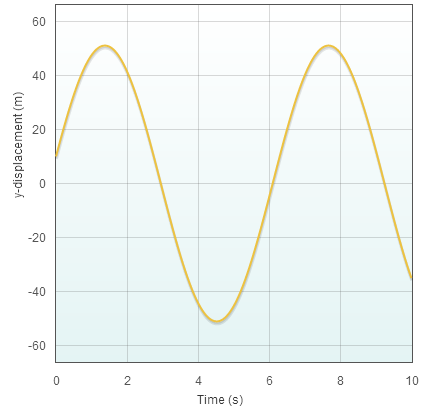
\includegraphics[width=\linewidth]{undamped_free.png}
 \captionof{figure}{Simulation of undamped free vibration with $m = 100$, $k = 100$, $y_0 = 10$, $v_0 = 50$, over the period $t = [0, 10]$}
\end{Figure}

As seen in Figure 1, an undamped free vibration is a sinusoidal wave which does not decay over time. 

\subsection {Damped Free Vibration}
Damped free vibrations are described by the homogenous differential equation $ay'' + by' +cy = 0$, and the general form of the vibration is $my'' + {\gamma}y' + ky = 0$. In this case, $\gamma$ is a positive damping term, $m$ is the mass, and $k$ is the spring constant.

The characteristic equation for this differential equation is $m{\lambda}^2 + {\gamma}{\lambda} + k = 0$. Because the coefficient, $\gamma$, can be non-zero, the characteristic equation will either have two real roots, one real root, or two complex roots.
\subsubsection {Overdamped Harmonic Motion}
If ${\gamma}^2 - 4mk > 0$, then the equation is solved with two real roots ${\lambda}_{1,2} = {\frac{-\gamma}{2m}} \pm \frac{\sqrt{{\gamma}^2 - 4mk}}{2m}$. Therefore by \eqref{eq:two_real_roots}, the general solution will be:

\begin{equation}\label{eq:overdamped_free}
y(t) = {y_0}e^{{\lambda}_1t} + \frac{v_0}{\omega}e^{{\lambda}_2t}
\end{equation}

Consider a block with a mass of 10 kg attached to a spring that stretches 1 meter for every 2.5 N of force applied to it. The block is also subject to a damping force with a constant damping coefficient $\gamma = 15$. When the block is initially displaced 10 m and the initial velocity of the block is set to 10 m/s, what will the position of the block be at time $t$?

Since we are given the constants $k = 2.5 N/m$, $m = 10 kg$, $y_0 = 10 m$, $v_0 = 10 m/s$, and $\gamma = 15$, we can simply substitute the constants into \eqref{eq:overdamped_free} to determine the position of the block at any time $t$. Note that $\omega = \sqrt{\frac{k}{m}} = \sqrt{\frac{2.5}{10}} = \frac{1}{2}$:

\begin{equation}
y(t) = 10e^{-0.191t} + 20e^{-1.309t}
\end{equation}

\begin{Figure}
 \centering
 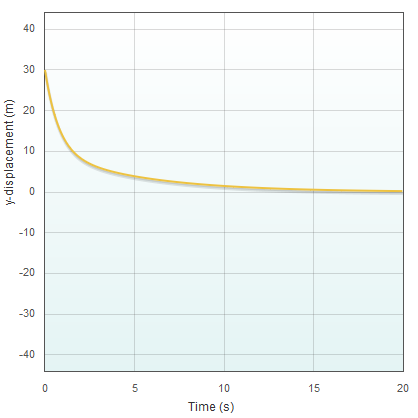
\includegraphics[width=\linewidth]{overdamped_free.png}
 \captionof{figure}{Simulation of overdamped free vibration with $m = 10$, $k = 2.5$, $\gamma = 15$, $y_0 = 10$, $v_0 = 10$, over the period $t = [0, 20]$}
\end{Figure}


\subsubsection {Critically Damped Harmonic Motion}
If ${\gamma}^2 = 4mk$, then the equation is solved with one real root ${\lambda}_1 = {\lambda}_2 = \frac{-\gamma}{2m}$. Therefore by \eqref{eq:one_real_root}, the general soution will be:
\begin{equation}\label{eq:critically_damped}
y(t) = (A + Bt)e^{{\frac{{-\gamma}t}{2m}}}	
\end{equation}

Consider a block with a mass of 10 kg attached to a spring that stretches 1 meter for every 2.5 N of force applied to it. The block is also subject to a damping force with a constant damping coefficient $\gamma = 10$. When the block is initially displaced 10 m and the initial velocity of the block is set to 10 m/s, what will the position of the block be at time $t$?

Since we are given the constants $k = 2.5 N/m$, $m = 10 kg$, $y_0 = 10 m$, $v_0 = 10 m/s$, and $\gamma = 10$, we can simply substitute the constants into \eqref{eq:critically_damped} to determine the position of the block at any time $t$. Note that $\omega = \sqrt{\frac{k}{m}} = \sqrt{\frac{2.5}{10}} = \frac{1}{2}$:

\begin{equation}
y(t) = (10 + 20t)e^{-0.5t}
\end{equation}

\begin{Figure}
 \centering
 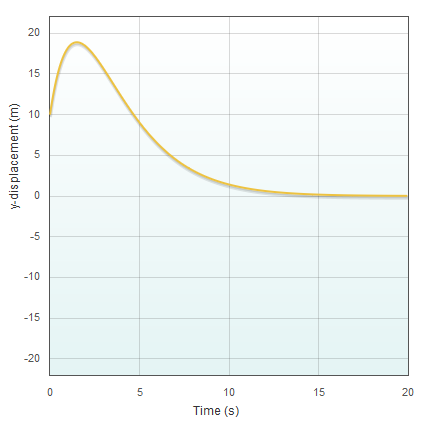
\includegraphics[width=\linewidth]{critically_damped_free.png}
 \captionof{figure}{Simulation of critically damped free vibration with $m = 10$, $k = 2.5$, $\gamma = 10$, $y_0 = 10$, $v_0 = 10$, over the period $t = [0, 20]$}
\end{Figure}

\subsubsection {Underdamped Harmonic Motion}
If ${\gamma}^2 - 4mk < 0$, then the equation is solved with two complex roots ${\lambda}_{1,2} = \frac{-\gamma}{2m} \pm iv$, where $v = \frac{\sqrt{4mk - {\gamma}^2}}{2m}$. Therefore by \eqref{eq:two_complex_roots}, the general solution will be:
\begin{equation}\label{eq:underdamped}
y(t) = e^{{\frac{-{\gamma}t}{2m}}}(Acos(vt) + Bsin(vt))
\end{equation}

Consider a block with a mass of 100 kg attached to a spring that stretches 1 meter for every 100 N of force applied to it. The block is also subject to a damping force with a constant damping coefficient $\gamma = 10$. When the block is initially displaced 10 m and the initial velocity of the block is 30 m/s, what will the position of the block be at time $t$?

Since we are given the constants $k = 100 N/m$, $m = 100 kg$, $y_0 = 10 m$, $v_0 = 30 m/s$, and $\gamma = 10$, we can simply substitute the constants into \eqref{eq:underdamped} to determine the position of the block at any time $t$. Note that $\omega = \sqrt{\frac{k}{m}} = \sqrt{\frac{100}{100}} = 1$:

\begin{equation}
y(t) = e^{-0.05}(10cos(0.999t) + sin(0.999t))
\end{equation}

\begin{Figure}
 \centering
 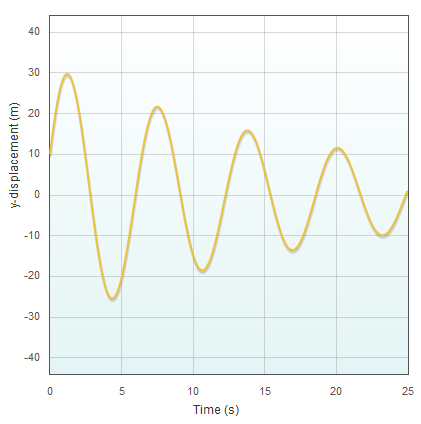
\includegraphics[width=\linewidth]{underdamped_free.png}
 \captionof{figure}{Simulation of underdamped free vibration with $m = 100$, $k = 100$, $\gamma = 10$, $y_0 = 10$, $v_0 = 30$, over the period $t = [0, 25]$}
\end{Figure}

\subsection {Forced Vibration}



\end{multicols}

\end{document}